\section{Experiments}
We conduct a comprehensive set of experiments to evaluate the effectiveness of our proposed method, \textit{Inference Scaled GraphRAG}, in enhancing multi-hop question answering on knowledge graphs. Specifically, we establish the following:

\begin{itemize}
    \item Inference-time scaling improves performance predictably on graph-based QA. 
    \item Our method improves performance across different levels of reasoning difficulty. We notably see improvements on questions that require multiple hops on the graph. 
    \item Our method performs favorably against traditional GraphRAG as well as previous graph traversal approaches.
\end{itemize}

% \begin{table*}[ht]
% \centering
% \caption{RougeL scores across domains for different majority voting thresholds and step counts.}
% \label{tab:scaling_results}
% \resizebox{\textwidth}{!}{
%     \begin{tabular}{lccccccccc c}
%     \toprule
%     \textbf{Config} & \textbf{Chemistry} & \textbf{Physics} & \textbf{Biology} & \textbf{Materials} & \textbf{Medicine} & \textbf{Amazon} & \textbf{DBLP} & \textbf{Biomedical} & \textbf{Goodreads} & \textbf{Avg} \\
%     \midrule
%     10 steps, votes=1  & 27.93 & 24.61 & 29.13 & 37.91 & 23.09 & 36.78 & 25.08 & 8.15 & 34.26 & 27.44 \\
%     25 steps, votes=1  & 40.26 & 28.64 & 28.64 & 30.90 & 23.29 & 36.55 & 26.22 & 5.43 & 33.22 & 28.13 \\
%     50 steps, votes=1  & 41.89 & 30.78 & 30.78 & 38.14 & 31.31 & 42.54 & 29.84 & 5.85 & 34.28 & 31.71 \\
%     \midrule
%     10 steps, votes=4  & 37.29 & 30.41 & 33.24 & 35.80 & 25.40 & 30.27 & 36.53 & 7.39 & 37.26 & 30.40 \\
%     25 steps, votes=4  & 41.41 & 29.78 & 32.00 & 43.32 & 32.30 & 34.75 & 34.39 & 11.98 & 40.56 & 33.39 \\
%     50 steps, votes=4  & 40.55 & 35.28 & 35.02 & 45.31 & 29.53 & 38.74 & 35.08 & 8.18 & 39.66 & 34.15 \\
%     \midrule
%     10 steps, votes=8  & 42.17 & 34.45 & 25.64 & 38.86 & 27.81 & 33.83 & 31.14 & 7.69 & 39.15 & 31.19 \\
%     25 steps, votes=8  & 40.84 & 33.07 & 34.88 & 41.88 & 31.88 & 41.74 & 32.57 & 11.74 & 39.46 & 34.23 \\
%     50 steps, votes=8  & 41.69 & 36.66 & 37.12 & 38.29 & 35.61 & 44.45 & 33.31 & 13.08 & 40.13 & 35.59 \\
%     \midrule
%     10 steps, votes=16 & 40.92 & 26.35 & 29.82 & 38.61 & 25.44 & 36.98 & 28.85 & 8.48 & 40.43 & 30.65 \\
%     25 steps, votes=16 & 42.81 & 31.47 & 37.25 & 35.46 & 32.91 & 37.98 & 34.63 & 9.07 & 40.89 & 33.61 \\
%     50 steps, votes=16 & 43.63 & 33.13 & 38.58 & 41.40 & 30.55 & 42.27 & 29.38 & 10.17 & 40.59 & 34.41 \\
%     \bottomrule
%     \end{tabular}
% }
% \end{table*}


% \begin{table*}[ht]
% \centering
% \caption{F1 scores across domains for different majority voting thresholds and step counts.}
% \label{tab:f1_scores}
%     \resizebox{\textwidth}{!}{
%     \begin{tabular}{lccccccc c}
%         \toprule
%         \textbf{Config} & \textbf{Chemistry} & \textbf{Physics} & \textbf{Biology} & \textbf{Materials} & \textbf{Medicine} & \textbf{Amazon} & \textbf{dblp} & \textbf{Avg} \\
%         \midrule
%         10 steps, votes=1  & 40.60 & 38.94 & 43.97 & 49.30 & 36.43 & 47.15 & 34.73 & 41.59 \\
%         25 steps, votes=1  & 57.40 & 46.69 & 46.69 & 48.36 & 43.46 & 52.42 & 42.64 & 48.24 \\
%         50 steps, votes=1  & 62.34 & 54.25 & 54.25 & 56.34 & 54.18 & 59.62 & 41.71 & 54.67 \\
%         \midrule
%         10 steps, votes=4  & 52.49 & 47.41 & 44.88 & 50.11 & 43.94 & 41.65 & 47.83 & 46.90 \\
%         25 steps, votes=4  & 61.76 & 54.40 & 50.53 & 62.54 & 57.83 & 51.27 & 49.30 & 55.38 \\
%         50 steps, votes=4  & 63.58 & 58.74 & 56.13 & 65.65 & 52.71 & 55.24 & 46.00 & 56.86 \\
%         \midrule
%         10 steps, votes=8  & 59.21 & 48.78 & 39.39 & 46.47 & 45.16 & 49.56 & 42.16 & 47.25 \\
%         25 steps, votes=8  & 62.32 & 53.75 & 50.84 & 61.00 & 54.57 & 58.73 & 50.40 & 55.94 \\
%         50 steps, votes=8  & 60.95 & 56.03 & 53.69 & 58.92 & 59.36 & 61.39 & 48.14 & 56.93 \\
%         \midrule
%         10 steps, votes=16 & 58.76 & 44.03 & 42.08 & 46.04 & 46.38 & 50.38 & 41.59 & 47.04 \\
%         25 steps, votes=16 & 63.68 & 49.93 & 53.26 & 55.26 & 54.59 & 54.26 & 50.57 & 54.51 \\
%         50 steps, votes=16 & 63.36 & 55.31 & 57.22 & 59.15 & 53.77 & 58.79 & 46.54 & 56.31 \\
%         \bottomrule 
%     \end{tabular}
%     }
% \end{table*}


\subsection{Benchmark dataset}

We evaluate our method on \textbf{GRBench} \citep{jin2024graph}, a knowledge graph-based question answering benchmark designed to assess multi-hop reasoning over structured data. GRBench includes a collection of domain-specific knowledge graphs spanning disciplines such as academic citations, e-commerce, literature, and healthcare. Each knowledge graph is paired with a set of natural language questions that require the model to retrieve and reason over relevant nodes and edges in the graph.

Questions are categorized into three difficulty levels based on the complexity of graph traversal and reasoning required to answer it:

\begin{itemize}
    \item \textbf{Easy}: Can be answered with a single node query or a one-hop traversal.
    \item \textbf{Medium}: Require multi-hop reasoning across several connected entities in the graph.
    \item \textbf{Hard}: Involve inductive or abstract reasoning, often requiring synthesizing multiple paths or patterns across the graph.
\end{itemize}

This structure makes GRBench an ideal benchmark for evaluating inference-time reasoning techniques, as it explicitly tests the model's ability to handle both shallow and deep reasoning tasks across diverse graph structures.

\subsection{Baselines and metrics}

We compare our approach with two categories of baselines:

\paragraph{GraphRAG}
We utilize an embedding model to retrieve semantically similar nodes and their surrounding subgraph. This text is fed to the LLM as context \citep{ye2024language}. We use standard 1 hop retrieval.

\paragraph{GraphCoT.}
the current state-of-the-art method for LLM-based graph traversal using function calls and reasoning steps. We retain their prompting style and retrieval mechanisms, and only vary the underlying model.

We adopt both symbolic and semantic evaluation metrics:

\begin{itemize}
    \item \textbf{RougeL:} Measures overlap based on the longest common subsequence between the generated answer and ground truth.
    \item \textbf{BERTScore (F1):} Uses BERT embeddings to compute token-level similarity between answers and references. We use DistilBERT-base-uncased for embedding generation.
\end{itemize}

\subsection{Implementation details}

All experiments are conducted on NVIDIA a100 and h100 GPUs using Python 3.9 and Huggingface Transformers v4.51.3. We use MPNet-v2 as the retriever and FAISS \citep{johnson2019billion} for indexing. Unless otherwise specified, Llama3.1-8B-Instruct serves as our main language model. We set temperature to 0.7 and utilize top-p sampling with a threshold of 0.9 to balance diversity and coherence in generated responses. Prompting templates and hyperparameters are provided in Appendix A.

We vary two inference scaling parameters to investigate the performance of both sequential and parallel inference scaling:
\begin{itemize}
    \item Number of reasoning steps. Scaling the number of reasoning steps corresponds to scaling inference sequentially. The LLM conditions the current generation on all previous thought action pairs.  
    \item Number of sampled thought-action pairs for majority voting. We utilize majority voting for our parallel scaling implementation in order to isolate the performance of inference scaling rather than utilizing an external reward model for verification.
\end{itemize}

% \subsection{Overall performance}

% We evaluate the overall effectiveness of Inference Scaled GraphRAG across a diverse set of domains in the GRBench benchmark, measuring F1 and RougeL performance under varying inference scaling configurations. Table \ref{tab:accuracy_votes_bold} and \ref{tab:llama8b-F1-scores} report RougeL and F1 results respectively averaged across nine domains, capturing a range of scientific, academic, and general purpose knowledge graphs. 

% Our findings demonstrate a clear and consistent trend: increasing inference budget, either through more reasoning steps (sequential scaling) or majority voting (parallel scaling) improves performance across all domains. Our method significantly outperforms standard GraphRAG approaches. 


% The base LLM achieves an average RougeL score of only $2.86\%$, GraphCoT, the previous state of the art graph reasoning method, achieves a RougeL score of $27\%$. Inference Scaled GraphRAG is able to achieve an F1 score of $35.59$, or a $28.57\%$ increase over GraphCoT. 

% Table \ref{tab:f1_scores} shows F1 scores by domain. Similarly, Inference Scaled GraphRAG is able to achieve an average F1 score of $53.33\%$ at maximum inference scaling settings compared to only $39.34\%$ with GraphCoT and $4\%$ with just the LLM. This represents an impressive $30.19\%$ improvement over GraphCoT. 

\begin{table*}[t]
\centering
\caption{F1 performance on the different domains of GRBench, comparing: (i) standard GraphRAG; (ii) GraphCoT with no inference scaling (equivalent to the Inference Scaled GraphRAG configuration of 10 steps and 1 vote); and (iii) Inference Scaled GraphRAG with varying step counts and majority voting thresholds. We adopt Llama3.1-8b-instruct as the model backbone for all presented results.}
\label{tab:llama8b-F1-scores}
    \resizebox{\textwidth}{!}{%
        \begin{tabular}{lccccccc}
        \toprule
        Inference config & \textbf{Academic} & \textbf{Amazon} & \textbf{DBLP} & \textbf{Biomedical} & \textbf{goodreads} & \textbf{Legal} & \textbf{Avg} \\
        \midrule
        GraphRAG & 33.71 & 38.34 & 28.01 & 11.29 & 37.26 & 28.56 & 28.87 \\
        \midrule
        10 steps, votes=1  & 41.85 & 47.15 & 34.73 & 8.66 & 48.81 & 32.27 & 36.49 \\
        25 steps, votes=1  & 48.52 & 52.42 & 42.64 & 11.55 & 53.24 & 32.27 & 40.11 \\
        50 steps, votes=1  & 56.27 & 59.62 & 41.71 & 12.26 & 52.94 & 35.33 & 43.02 \\
        \midrule
        10 steps, votes=4  & 47.77 & 41.65 & 47.83 & 12.33 & 53.28 & 34.09 & 39.49 \\
        25 steps, votes=4  & 57.41 & 51.27 & 49.30 & 19.02 & 60.25 & 33.97 & 45.20 \\
        50 steps, votes=4  & 57.76 & 55.24 & 46.00 & 15.58 & 57.35 & 34.46 & 44.67 \\
        \midrule
        10 steps, votes=8  & 47.80 & 49.56 & 42.16 & 14.70 & 54.42 & 36.61 & 40.88 \\
        25 steps, votes=8  & 56.50 & 58.73 & 50.40 & 19.19 & 58.76 & 26.32 & 44.98 \\
        50 steps, votes=8  & 57.79 & \textbf{61.39} & 48.14 & 18.94 & \textbf{61.91} & 34.56 & 47.12 \\
        \midrule
        10 steps, votes=16 & 47.46 & 50.38 & 41.59 & 13.11 & 53.33 & 30.35 & 39.37 \\
        25 steps, votes=16 & 55.34 & 54.26 & \textbf{50.57} & 16.28 & 58.65 & 36.84 & 45.32 \\
        50 steps, votes=16 & \textbf{59.36} & 58.79 & 46.54 & \textbf{19.55} & 61.80 & \textbf{40.88} & \textbf{47.55} \\
        \bottomrule
        \end{tabular}%
     }
\end{table*}

\subsection{Overall performance}

We evaluate the overall effectiveness of Inference Scaled GraphRAG across a diverse set of domains in the GRBench benchmark, measuring F1 and RougeL performance under varying inference scaling configurations. Table~\ref{tab:accuracy_votes_bold} (RougeL scores) and Table~\ref{tab:llama8b-F1-scores} (F1 scores) report these respective results, averaged across nine domains that capture a range of scientific, academic, and general-purpose knowledge graphs.

Our findings demonstrate a clear and consistent trend: increasing the inference budget, either through more reasoning steps (sequential scaling) or by employing majority voting over sampled trajectories (parallel scaling), systematically improves performance across all domains.

Inference Scaled GraphRAG significantly outperforms standard GraphRAG approaches. In terms of RougeL scores (Table~\ref{tab:accuracy_votes_bold}), the standard GraphRAG baseline achieves an average of $6.01$. The base configuration of Inference Scaled GraphRAG (10 steps, 1 vote), which is equivalent to GraphCoT with no inference scaling, achieves an average RougeL score of $27.21$. Performance is further enhanced with increased inference scaling, reaching an average RougeL score of up to $34.33$. 
Similarly, for F1 scores (Table~\ref{tab:llama8b-F1-scores}), Inference Scaled GraphRAG demonstrates substantial improvements. Standard GraphRAG achieves an average F1 score of $28.87$. GraphCoT improves on this with $36.49$, while our method reaches $47.55$ under the highest inference budget. observed in our experiments (configuration: 50 steps, 16 votes). These results underscore the benefits of inference-time compute scaling for enhancing graph-based question answering.



% \begin{table*}[ht]
% \centering
% \caption{F1 scores across domains for different majority voting thresholds and step counts.}
% \label{tab:f1_scores}
%     \resizebox{\textwidth}{!}{
%     \begin{tabular}{lccccccc c}
%         \toprule
%         \textbf{Config} & \textbf{Chemistry} & \textbf{Physics} & \textbf{Biology} & \textbf{Materials} & \textbf{Medicine} & \textbf{Amazon} & \textbf{dblp} & \textbf{Avg} \\
%         \midrule
%         10 steps, votes=1  & 40.60 & 38.94 & 43.97 & 49.30 & 36.43 & 47.15 & 34.73 & 41.59 \\
%         25 steps, votes=1  & 57.40 & 46.69 & 46.69 & 48.36 & 43.46 & 52.42 & 42.64 & 48.24 \\
%         50 steps, votes=1  & 62.34 & 54.25 & 54.25 & 56.34 & 54.18 & 59.62 & 41.71 & 54.67 \\
%         \midrule
%         10 steps, votes=4  & 52.49 & 47.41 & 44.88 & 50.11 & 43.94 & 41.65 & 47.83 & 46.90 \\
%         25 steps, votes=4  & 61.76 & 54.40 & 50.53 & 62.54 & 57.83 & 51.27 & 49.30 & 55.38 \\
%         50 steps, votes=4  & 63.58 & 58.74 & 56.13 & 65.65 & 52.71 & 55.24 & 46.00 & 56.86 \\
%         \midrule
%         10 steps, votes=8  & 59.21 & 48.78 & 39.39 & 46.47 & 45.16 & 49.56 & 42.16 & 47.25 \\
%         25 steps, votes=8  & 62.32 & 53.75 & 50.84 & 61.00 & 54.57 & 58.73 & 50.40 & 55.94 \\
%         50 steps, votes=8  & 60.95 & 56.03 & 53.69 & 58.92 & 59.36 & 61.39 & 48.14 & 56.93 \\
%         \midrule
%         10 steps, votes=16 & 58.76 & 44.03 & 42.08 & 46.04 & 46.38 & 50.38 & 41.59 & 47.04 \\
%         25 steps, votes=16 & 63.68 & 49.93 & 53.26 & 55.26 & 54.59 & 54.26 & 50.57 & 54.51 \\
%         50 steps, votes=16 & 63.36 & 55.31 & 57.22 & 59.15 & 53.77 & 58.79 & 46.54 & 56.31 \\
%         \bottomrule 
%     \end{tabular}
%     }
% \end{table*}

% \begin{table*}[ht]
% \centering
% \caption{F1 performance on the different domains of GRBench, comparing: (i) standard GraphRAG; (ii) GraphCoT with no inference scaling (equivalent to the Inference Scaled GraphRAG configuration of 10 steps and 1 vote); and (iii) Inference Scaled GraphRAG with varying step counts and majority voting thresholds. We adopt Llama3.1-8b-instruct as the model backbone for all presented results.}
% \label{tab:llama8b-F1-scores}
%     \resizebox{\textwidth}{!}{%
%         \begin{tabular}{lccccccc}
%         \toprule
%         Inference config & \textbf{Academic} & \textbf{Amazon} & \textbf{DBLP} & \textbf{Biomedical} & \textbf{goodreads} & \textbf{Legal} & \textbf{Avg} \\
%         \midrule
%         GraphRAG & - & - & - & - & - & - & \\
%         \midrule
%         10 steps, votes=1  & 41.85 & 47.15 & 34.73 & 14.14 & 48.81 & 32.27 & 36.49 \\
%         25 steps, votes=1  & 48.52 & 52.42 & 42.64 & 11.55 & 53.24 & 32.27 & 40.11 \\
%         50 steps, votes=1  & 56.27 & 59.62 & 41.71 & 12.26 & 52.94 & 35.33 & 43.02 \\
%         \midrule
%         10 steps, votes=4  & 47.77 & 41.65 & 47.83 & 12.33 & 53.28 & 34.09 & 39.49 \\
%         25 steps, votes=4  & 57.41 & 51.27 & 49.30 & 19.02 & 60.25 & 33.97 & 45.20 \\
%         50 steps, votes=4  & 59.36 & 55.24 & 46.00 & 15.58 & 57.35 & 34.46 & 44.67 \\
%         \midrule
%         10 steps, votes=8  & 47.80 & 49.56 & 42.16 & 14.70 & 54.42 & 36.61 & 40.88 \\
%         25 steps, votes=8  & 56.50 & 58.73 & 50.40 & 19.19 & 58.76 & 26.32 & 44.98 \\
%         50 steps, votes=8  & 57.79 & 61.39 & 48.14 & 18.94 & 61.91 & 34.56 & 47.12 \\
%         \midrule
%         10 steps, votes=16 & 47.46 & 50.38 & 41.59 & 13.11 & 53.33 & 30.35 & 39.37 \\
%         25 steps, votes=16 & 55.34 & 54.26 & 50.57 & 16.28 & 58.65 & 36.84 & 45.32 \\
%         50 steps, votes=16 & 57.76 & 58.79 & 46.54 & 19.55 & 61.80 & 40.88 & 47.55 \\
%         \bottomrule
%         \end{tabular}%
% tot     }
% \end{table*}

% \begin{table*}[t]
%     \centering
%     \caption{Rouge-L performance on the different domains of GRBench, comparing: (i) standard GraphRAG; (ii) GraphCoT with no inference scaling (equivalent to the Inference Scaled GraphRAG configuration of 10 steps and 1 vote); and (iii) Inference Scaled GraphRAG with varying step counts and majority voting thresholds. We adopt Llama3.1-8b-instruct as the model backbone for all presented results.}
%         \resizebox{\textwidth}{!}{%
%         \begin{tabular}{lccccccc}
%         \toprule
%         Inference config & \textbf{Academic} & \textbf{Amazon} & \textbf{DBLP} & \textbf{Biomedical} & \textbf{Goodreads} & \textbf{Legal} & \textbf{Avg} \\
%         \midrule
%         GraphRAG & 8.99 & 8.54 & 6.94 & 3.30 & 3.01 & 5.28 & 6.01 \\
%         \midrule
%         10 steps, votes=1  & 28.53 & 36.78 & 25.08 & 8.15  & 34.26 & 25.11 & 27.21 \\
%         25 steps, votes=1  & 30.35 & 36.55 & 26.22 & 5.43  & 33.22 & 24.06 & 27.72 \\
%         50 steps, votes=1  & 34.58 & 42.54 & 29.84 & 5.85  & 34.28 & 25.30 & 31.07 \\
%         \midrule
%         10 steps, votes=4  & 32.43 & 30.27 & 29.38 & 7.39  & 37.26 & 26.45 & 30.00 \\
%         25 steps, votes=4  & 35.76 & 34.75 & 34.39 & 11.98 & 40.56 & 24.29 & 32.48 \\
%         50 steps, votes=4  & 37.14 & 38.74 & 35.08 & 8.18  & 39.66 & 22.51 & 32.99 \\
%         \midrule
%         10 steps, votes=8  & 33.79 & 33.83 & 31.14 & 7.69  & 39.15 & 24.88 & 30.56 \\
%         25 steps, votes=8  & 36.51 & 41.74 & 32.57 & 11.74 & 39.46 & 16.54 & 32.46 \\
%         50 steps, votes=8  & 37.87 & 44.45 & 33.31 & 13.08 & 40.13 & 22.99 & 34.33 \\
%         \midrule
%         10 steps, votes=16 & 32.23 & 36.98 & 28.85 & 8.48  & 40.43 & 20.95 & 29.68 \\
%         25 steps, votes=16 & 35.98 & 37.98 & 34.63 & 9.07  & 40.89 & 27.24 & 32.97 \\
%         50 steps, votes=16 & 37.46 & 42.27 & 36.53 & 10.17 & 40.59 & 28.48 & 33.82 \\
%         \bottomrule
%         \end{tabular}%
%         }
% \label{tab:accuracy_votes_bold}
% \end{table*}

\begin{table*}[t]
    \centering
    \caption{RougeL performance on the different domains of GRBench, comparing: (i) standard GraphRAG; (ii) GraphCoT with no inference scaling (equivalent to the Inference Scaled GraphRAG configuration of 10 steps and 1 vote); and (iii) Inference Scaled GraphRAG with varying step counts and majority voting thresholds. We adopt Llama3.1-8b-instruct as the model backbone for all presented results.}
        \resizebox{\textwidth}{!}{%
        \begin{tabular}{lccccccc}
        \toprule
        Inference config & \textbf{Academic} & \textbf{Amazon} & \textbf{DBLP} & \textbf{Biomedical} & \textbf{Goodreads} & \textbf{Legal} & \textbf{Avg} \\
        \midrule
        GraphRAG & 8.99 & 8.54 & 6.94 & 3.30 & 3.01 & 5.28 & 6.01 \\
        \midrule
        10 steps, votes=1  & 28.53 & 36.78 & 25.08 & 8.15  & 34.26 & 25.11 & 27.21 \\
        25 steps, votes=1  & 30.35 & 36.55 & 26.22 & 5.43  & 33.22 & 24.06 & 27.72 \\
        50 steps, votes=1  & 34.58 & 42.54 & 29.84 & 5.85  & 34.28 & 25.30 & 31.07 \\
        \midrule
        10 steps, votes=4  & 32.43 & 30.27 & 29.38 & 7.39  & 37.26 & 26.45 & 30.00 \\
        25 steps, votes=4  & 35.76 & 34.75 & 34.39 & 11.98 & 40.56 & 24.29 & 32.48 \\
        50 steps, votes=4  & 37.14 & 38.74 & 35.08 & 8.18  & 39.66 & 22.51 & 32.99 \\
        \midrule
        10 steps, votes=8  & 33.79 & 33.83 & 31.14 & 7.69  & 39.15 & 24.88 & 30.56 \\
        25 steps, votes=8  & 36.51 & 41.74 & 32.57 & 11.74 & 39.46 & 16.54 & 32.46 \\
        50 steps, votes=8  & 37.46 & \textbf{44.45} & 33.31 & \textbf{13.08} & 40.13 & 22.99 & 33.82 \\
        \midrule
        10 steps, votes=16 & 32.23 & 36.98 & 28.85 & 8.48  & 40.43 & 20.95 & 29.68 \\
        25 steps, votes=16 & 35.98 & 37.98 & 34.63 & 9.07  & 40.59 & 27.24 & 32.97 \\
        50 steps, votes=16 & \textbf{37.87} & 42.27 & \textbf{36.53} & 10.17 & \textbf{40.89} & \textbf{28.48} & \textbf{34.33} \\
        \bottomrule
        \end{tabular}%
        }
\label{tab:accuracy_votes_bold}
\end{table*}



% \begin{table*}[ht]
% \centering
% \caption{RougeL scores across domains for different majority voting thresholds and step counts.}
% \label{tab:scaling_results}
% \resizebox{\textwidth}{!}{
%     \begin{tabular}{lccccccccc c}
%     \toprule
%     \textbf{Config} & \textbf{Chemistry} & \textbf{Physics} & \textbf{Biology} & \textbf{Materials} & \textbf{Medicine} & \textbf{Amazon} & \textbf{DBLP} & \textbf{Biomedical} & \textbf{Goodreads} & \textbf{Avg} \\
%     \midrule
%     10 steps, votes=1  & 27.93 & 24.61 & 29.13 & 37.91 & 23.09 & 36.78 & 25.08 & 8.15 & 34.26 & 27.44 \\
%     25 steps, votes=1  & 40.26 & 28.64 & 28.64 & 30.90 & 23.29 & 36.55 & 26.22 & 5.43 & 33.22 & 28.13 \\
%     50 steps, votes=1  & 41.89 & 30.78 & 30.78 & 38.14 & 31.31 & 42.54 & 29.84 & 5.85 & 34.28 & 31.71 \\
%     \midrule
%     10 steps, votes=4  & 37.29 & 30.41 & 33.24 & 35.80 & 25.40 & 30.27 & 36.53 & 7.39 & 37.26 & 30.40 \\
%     25 steps, votes=4  & 41.41 & 29.78 & 32.00 & 43.32 & 32.30 & 34.75 & 34.39 & 11.98 & 40.56 & 33.39 \\
%     50 steps, votes=4  & 40.55 & 35.28 & 35.02 & 45.31 & 29.53 & 38.74 & 35.08 & 8.18 & 39.66 & 34.15 \\
%     \midrule
%     10 steps, votes=8  & 42.17 & 34.45 & 25.64 & 38.86 & 27.81 & 33.83 & 31.14 & 7.69 & 39.15 & 31.19 \\
%     25 steps, votes=8  & 40.84 & 33.07 & 34.88 & 41.88 & 31.88 & 41.74 & 32.57 & 11.74 & 39.46 & 34.23 \\
%     50 steps, votes=8  & 41.69 & 36.66 & 37.12 & 38.29 & 35.61 & 44.45 & 33.31 & 13.08 & 40.13 & 35.59 \\
%     \midrule
%     10 steps, votes=16 & 40.92 & 26.35 & 29.82 & 38.61 & 25.44 & 36.98 & 28.85 & 8.48 & 40.43 & 30.65 \\
%     25 steps, votes=16 & 42.81 & 31.47 & 37.25 & 35.46 & 32.91 & 37.98 & 34.63 & 9.07 & 40.89 & 33.61 \\
%     50 steps, votes=16 & 43.63 & 33.13 & 38.58 & 41.40 & 30.55 & 42.27 & 29.38 & 10.17 & 40.59 & 34.41 \\
%     \bottomrule
%     \end{tabular}
% }
% \end{table*}


\subsection{Different LLM backbones}
To understand how our method interacts with different language model sizes and architectures, we evaluate our method with two additional LLM backbones: Mixtral-8x7B-Instruct-v0.1 and Qwen3-32b. These models allow us to assess the generality and robustness of our approach. 

Table \ref{tab:average-f1-rouge} demonstrates that both Mixtral and Qwen3 benefit substantially from increased inference scaling. Performance consistently improves as the number of reasoning steps increases, confirming that deeper graph exploration enhances multi-hop reasoning capabilities irrespective of the underlying LLM backbone.

Notably, Qwen3-32b exhibits the most pronounced gains. While baseline performance across Mixtral-8x7B, Llama3.1-8B, and Qwen3-32b is comparable, with each achieving an F1 score near $37$, Qwen3-32b attains an F1 score approaching $64$ at maximum inference scaling. In contrast, Mixtral’s performance peaks at approximately $49.44$ under the same conditions. This disparity suggests that Qwen3 32b’s stronger inherent reasoning ability enables more effective knowledge graph traversal and information synthesis when augmented with inference time scaling. 

\begin{table*}[ht]
\centering
\caption{Average F1 and RougeL scores for Qwen3-32b and Mixtral-8x7b-Instruct across various configurations.}
\label{tab:average-f1-rouge}
\begin{tabular}{lcccc}
\toprule
& \multicolumn{2}{c}{\textbf{F1 Score}} & \multicolumn{2}{c}{\textbf{RougeL Score}} \\
\textbf{\begin{tabular}[c]{@{}l@{}}Configuration\end{tabular}} & Qwen & Mixtral & Qwen & Mixtral \\
\midrule
10 steps, 1 vote & 36.56 & 38.30 & 27.76 & 25.19 \\
25 steps, 1 vote & 53.00 & 45.88 & 35.85 & 30.45 \\
50 steps, 1 vote & 58.60 & 48.01 & 40.89 & 30.68 \\
\midrule
10 steps, 4 votes & 37.36 & 41.41 & 28.00 & 27.23 \\
25 steps, 4 votes & 52.96 & 45.71 & 36.63 & 28.90 \\
50 steps, 4 votes & 56.98 & 47.58 & 37.99 & 30.32 \\
\midrule
10 steps, 8 votes & 37.65 & 41.86 & 28.15 & 28.33 \\
25 steps, 8 votes & 58.39 & 48.56 & 39.23 & 30.05 \\
50 steps, 8 votes & 61.80 & 46.73 & 42.47 & 31.67 \\
\midrule
10 steps, 16 votes & 40.18 & 43.29 & 30.29 & 28.86 \\
25 steps, 16 votes & 57.98 & 46.94 & 40.11 & 30.36 \\
50 steps, 16 votes & \textbf{63.99} & \textbf{49.44} & \textbf{45.60} & \textbf{32.10} \\
\bottomrule
\end{tabular}
\end{table*}




\subsection{Effect of inference scaling by question difficulty}

To evaluate the impact of inference scaling on multi-hop reasoning, we analyze RougeL and F1 scores on a subset of the questions in GRBench  denoted as {\it medium} and {\it hard}. Figure \ref{fig:multi-hopf1} illustrates the performance improvements achieved by significantly increasing the inference budget (50 steps, 16 votes) over baseline (10 steps, 1 vote). 

We observe that increasing inference compute significantly improves the model's ability to perform multi-hop reasoning. Performance improves by $18.82\%$ on average across domains and $23.27\%$ at most suggesting that with more inference compute the model is able to more effectively explore the graph and retrieve relevant information.

We observe that sequential scaling is the primary driver of performance improvement on these problems, with parallel scaling providing a modest performance boost. We attribute this to the fact that parallel scaling does not directly impact the ability of the model to explore relationships in the graph. For example, a question that can be answered by retrieving relevant information from a node within the local subgraph 3 steps away requires the LLM to generate at least six thought action pairs leaving little room for the LLM to fully explore the subgraph. 

These findings highlight two key takeaways: (1) deeper inference directly improves the multi hop reasoning abilities of LLMs by allowing the model to effectively explore local structure (2) parallel scaling serves as a complementary strategy that improves robustness when applied in conjunction with deep reasoning. Together, these results reinforce the importance of inference time compute allocation in enhancing the symbolic reasoning capacity of LLMs over structured knowledge graphs.




% \subsection{Effect of Inference Scaling by Question Difficulty}

% To evaluate the impact of inference-time scaling on multi-hop reasoning performance, we analyze ROUGE-L and F1 scores on a subset of the GRBench dataset categorized as \textit{medium} and \textit{hard} questions. These subsets are designed to require multi-hop traversal or inductive reasoning across multiple entities and relations in the knowledge graph. Figure shows ROUGE-L performance as a function of reasoning steps, across various majority voting thresholds.

% We observe that increasing the number of inference steps significantly enhances the model's ability to answer medium and hard questions. In particular, performance improves by more than 20\% as the number of steps increases from 10 to 50, highlighting the benefit of deeper sequential reasoning. This trend confirms that additional inference compute enables the model to traverse a broader portion of the graph and synthesize information across multiple hops.

% Incorporating parallel scaling through majority voting further boosts performance, particularly at moderate voting thresholds (e.g., $k=4$ or $k=8$). However, we observe diminishing returns for higher thresholds ($k>8$), which we attribute to the limitations of the underlying LLM (Llama3.1-8B). Specifically, when the base model's reasoning traces lack sufficient diversity or quality, additional sampling provides limited benefit.

% Moreover, our analysis suggests that parallel scaling is less effective for questions requiring long, compositional reasoning chains. Because each sampled response is generated independently, majority voting tends to favor shorter, more common trajectories rather than exploring the full reasoning space. For instance, answering a question that requires synthesizing facts three hops apart often demands at least six well-aligned thought-action pairs. Without sufficient depth in each sample, parallel scaling alone fails to access the relevant information.

% These findings support two key takeaways: (1) increasing the number of reasoning steps (sequential scaling) plays a dominant role in improving multi-hop question answering, and (2) parallel scaling serves as a complementary strategy that improves robustness when applied in conjunction with deep reasoning. Together, these results reinforce the importance of inference-time compute allocation in enhancing the symbolic reasoning capacity of LLMs over structured knowledge graphs.


% \begin{figure}[t]
% \centering
%     \begin{subfigure}[t]{0.48\textwidth}
%         \centering
%         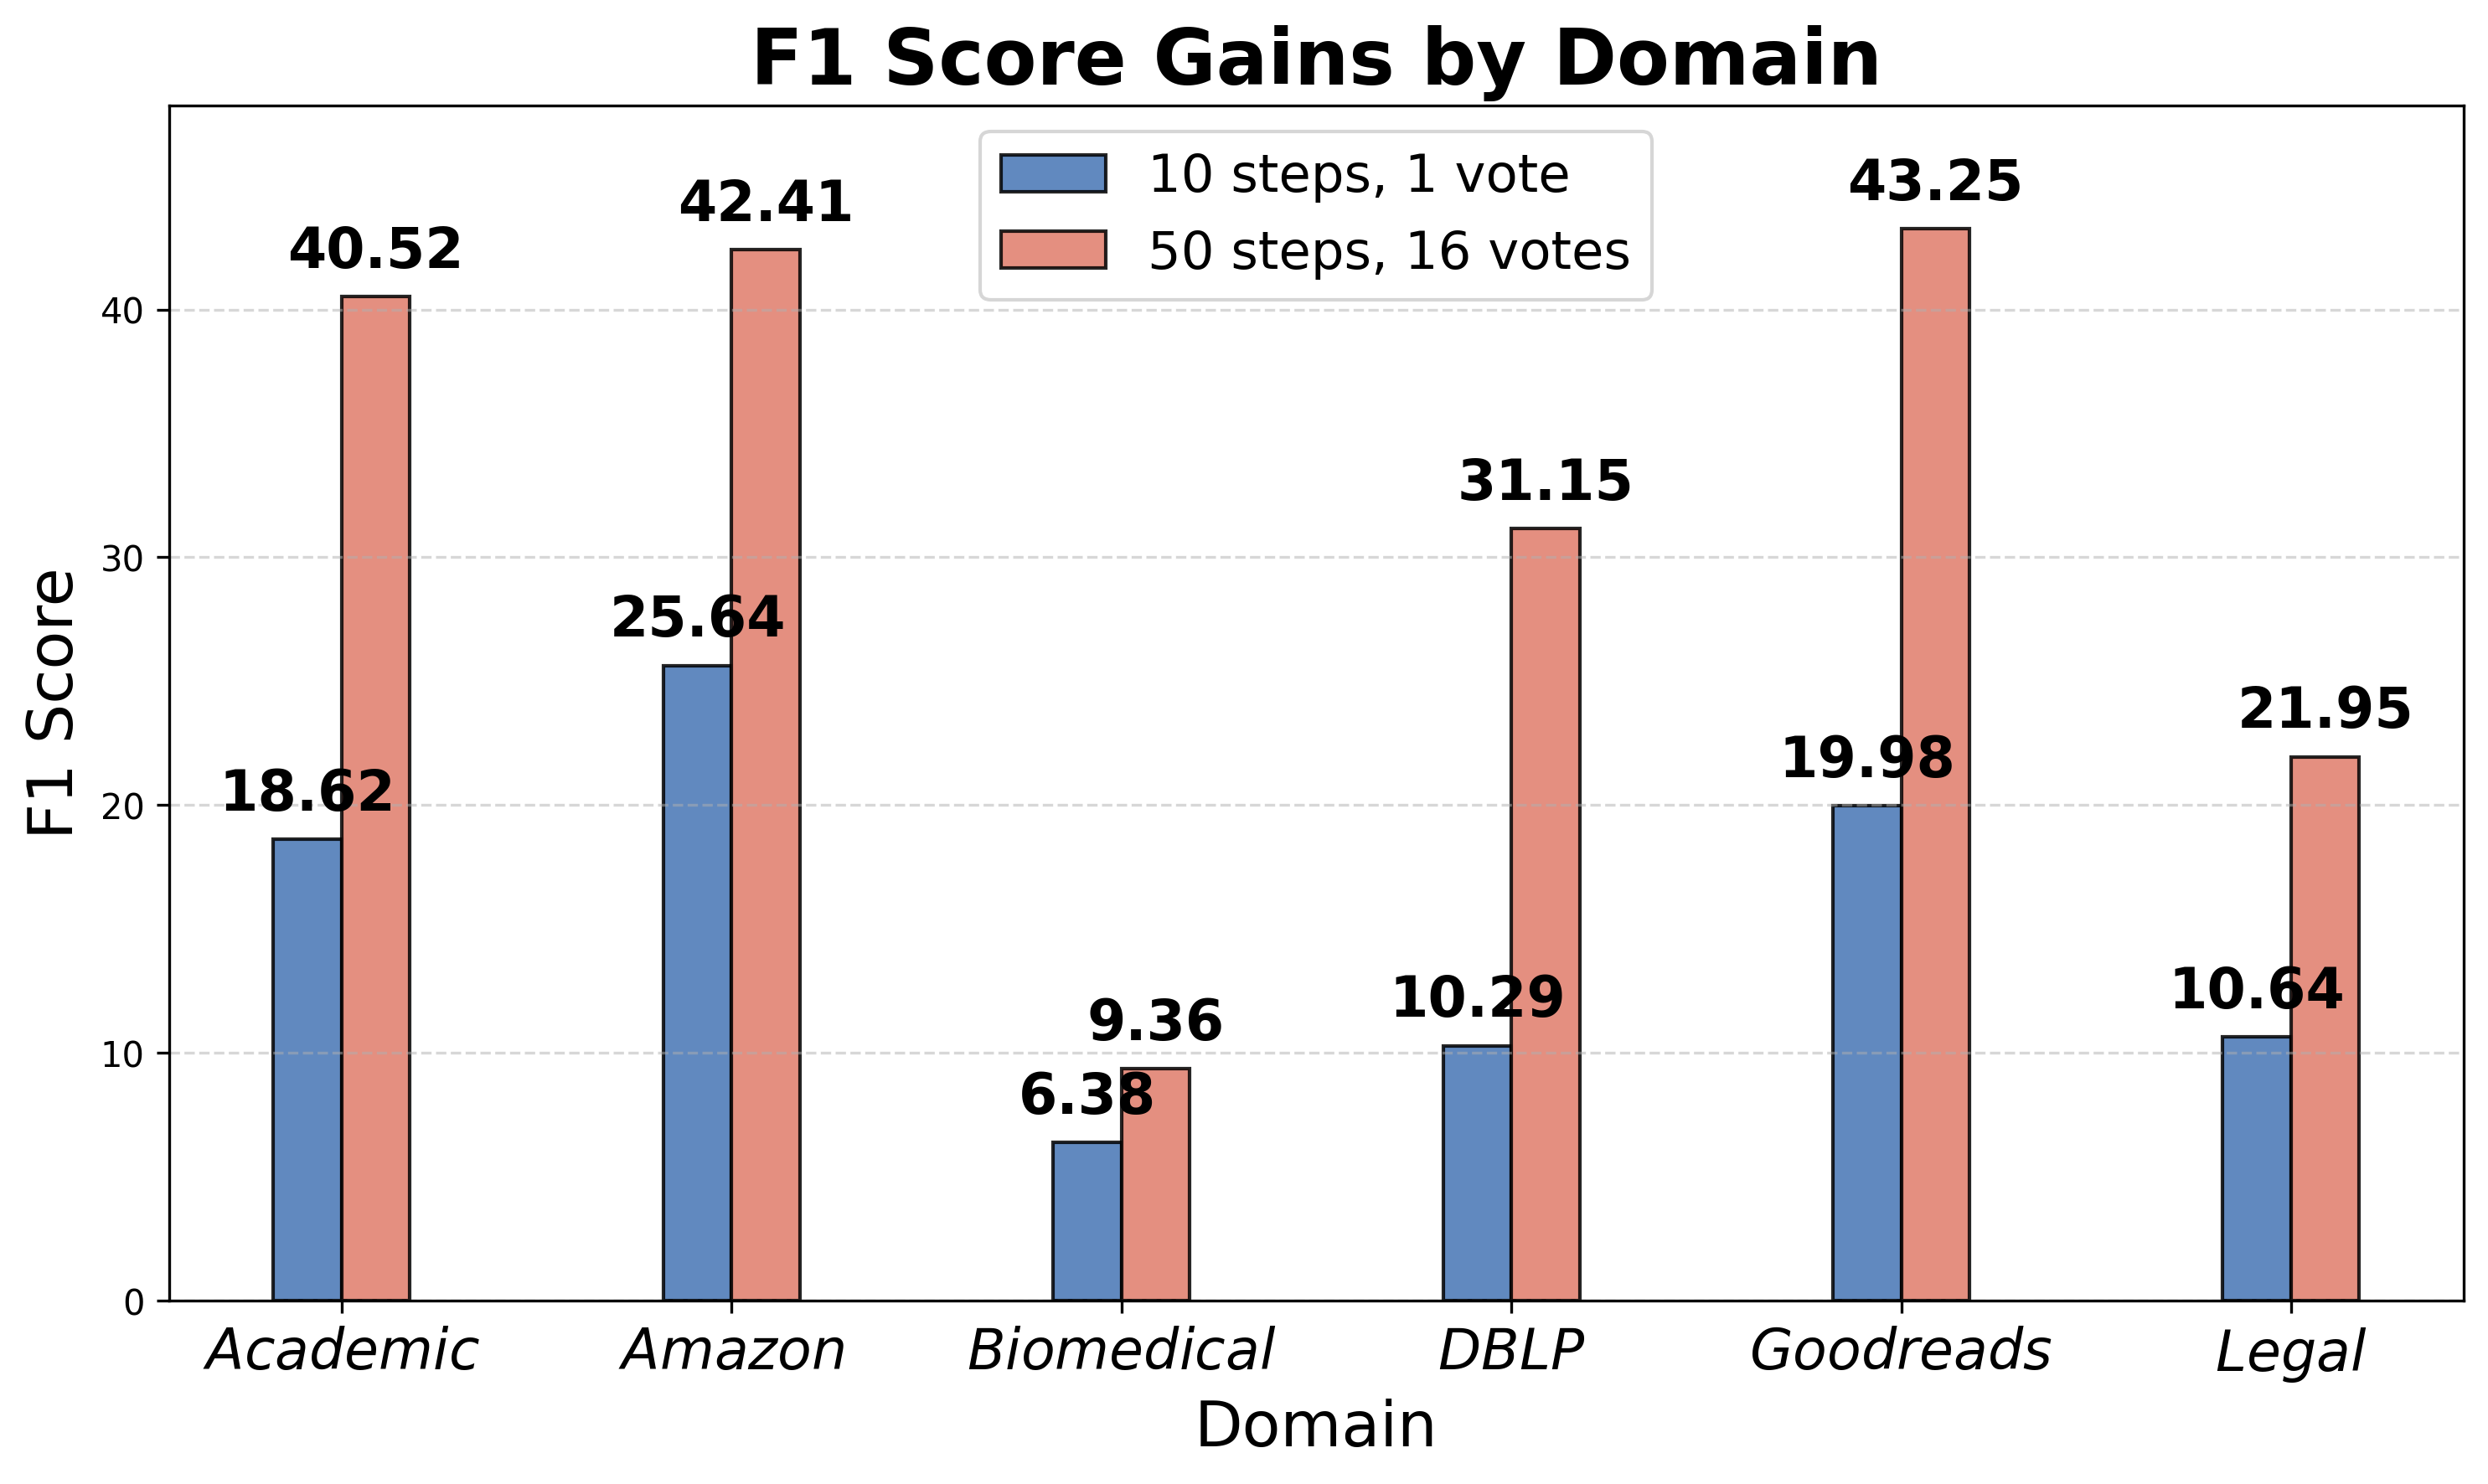
\includegraphics[width=\textwidth]{img/f1_score_medium_hard_avg_domain_bar_chart.png}
%         \caption{F1 scores on medium and hard questions}
%         \label{fig:multi-hopf1}
%     \end{subfigure}
%     \begin{subfigure}[t]{0.48\textwidth}
%         \centering
%         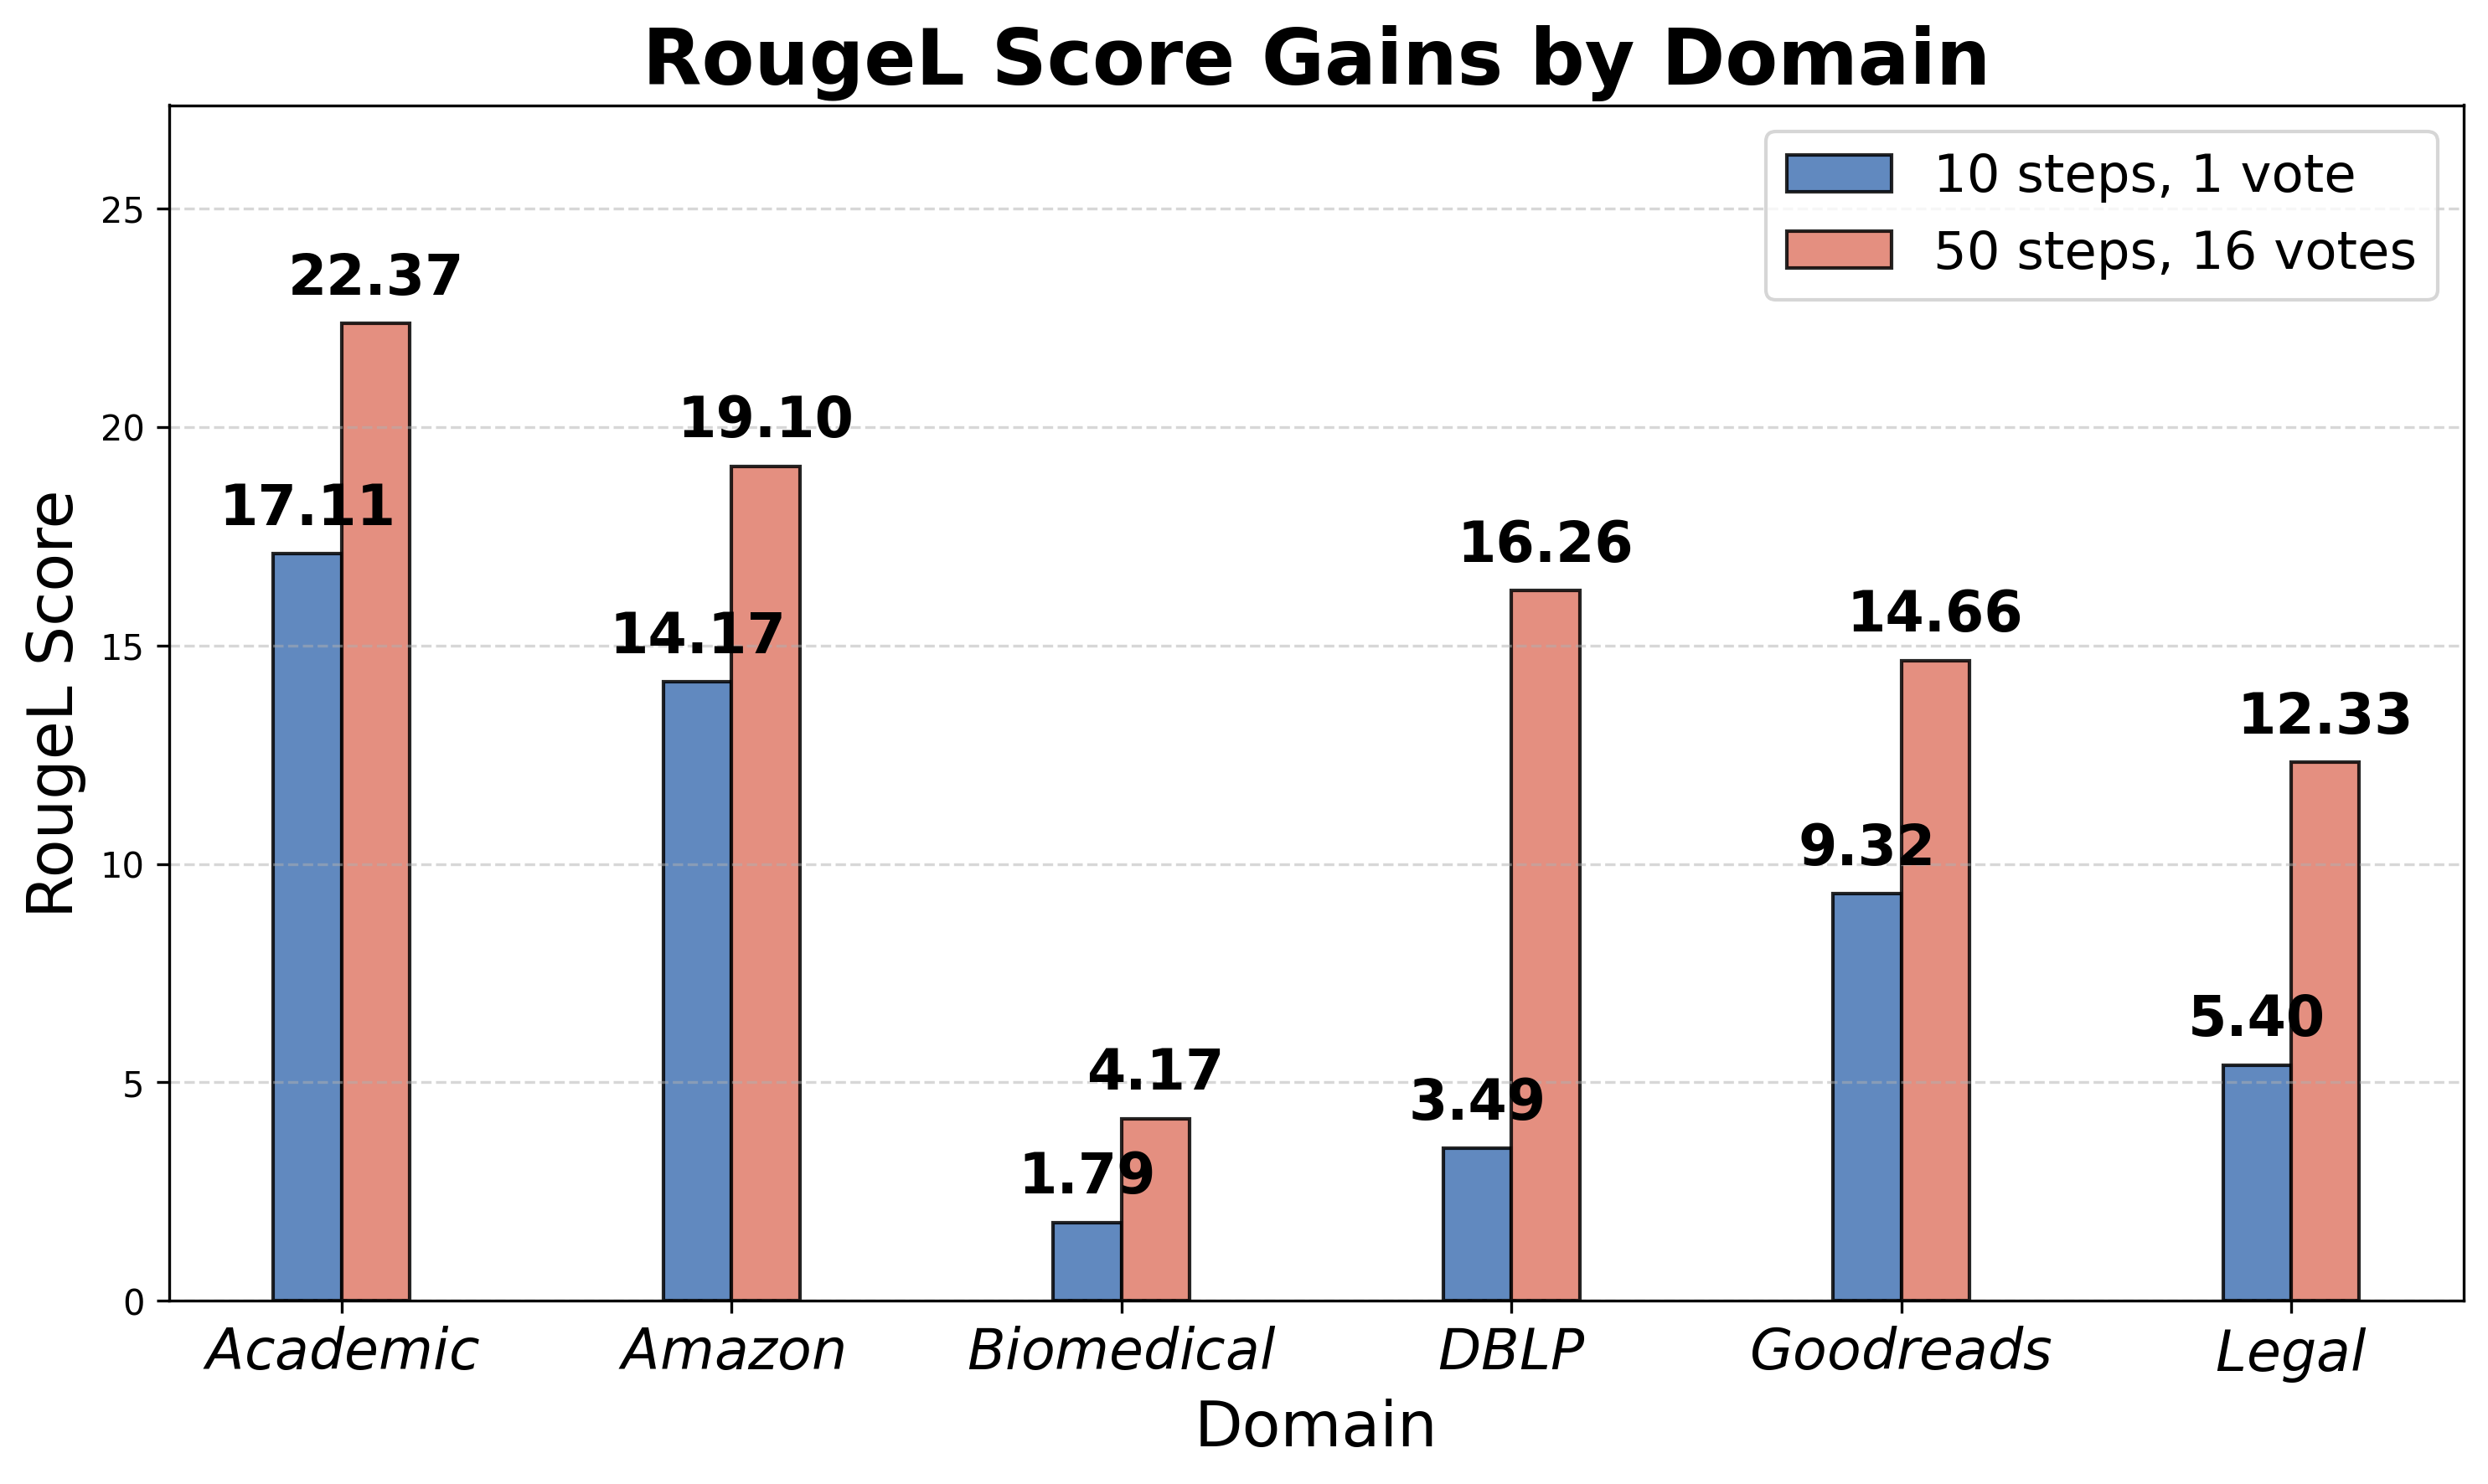
\includegraphics[width=\textwidth]{img/rougel_medium_hard_avg_domain_bar_chart.png}
%         \caption{RougeL scores on medium and hard questions}
%         \label{fig:multi-hoprougl}
%     \end{subfigure}
%     \caption{Performance improvements across domains with maximum inference scaling (50 steps, 16 votes) compared to no inference scaling (10 steps, 1 vote). Subfigure (a) reports F1 score gains on medium and hard questions, while (b) shows corresponding improvements in RougeL score. The results demonstrate consistent and substantial gains across all six domains, highlighting the effectiveness of inference scaling for complex question answering }
% \end{figure}

\subsection{Sequential vs parallel scaling}

To better understand the contributions of sequential and parallel inference scaling, we perform an ablation study comparing their isolated and combined effects.

Increasing the number of reasoning steps (i.e. thought action pairs), allows the model to iteratively explore the knowledge graph. This deeper traversal improves multi-hop reasoning by enabling the model to gather and integrate evidence across distant nodes. In table \ref{tab:llama8b-F1-scores}, increasing the step count from 10 to 50 while holding the number of sampled responses constant (votes = 1) led to an average F1 score improvement of $6.53\%$ and a maximum improvement of $14.42\%$, demonstrating the clear benefits of sequential scaling.  

We observe that parallel scaling offers modest performance improvements and primarily boosts robustness against individual errors capturing a wider range of actions. Table \ref{tab:llama8b-F1-scores} shows parallel scaling improves performance by $4.39\%$ on average and $6.86\%$ at most. Parallel scaling is most effective when the base model is already capable of generating high quality reasoning steps. Future work may aim to improve the performance of parallel scaling by utilizing alternative parallel scaling methods such as Best-of-N.

% Parallel scaling relies on generating multiple candidate actions and selecting the final answer via majority voting. While this strategy boosts robustness against individual errors and captures a wider range of actions, we observe diminishing returns beyond a moderate number of samples. For instance, increasing the number of votes from 1 to 4 consistently improves performance across step counts, but increasing from 8 to 16 provides marginal gains at best \ref{tab:f1_scores}. This suggests that parallel sampling is most effective when the base model is already capable of generating high quality reasoning steps. Future work may aim to improve the performance of parallel scaling by utilizing alternative parallel scaling methods such as Best-of-N. 

When combined, sequential scaling and parallel scaling yield the highest performance, especially on medium and hard questions requiring multi-hop reasoning. This suggests a synergistic effect where sequential scaling provides the necessary depth exploration and iterative reasoning, while parallel scaling enhances consistency, reliability, and robustness of the final output.

\begin{figure}[t]
\centering
    \begin{subfigure}[t]{0.48\textwidth}
        \centering
        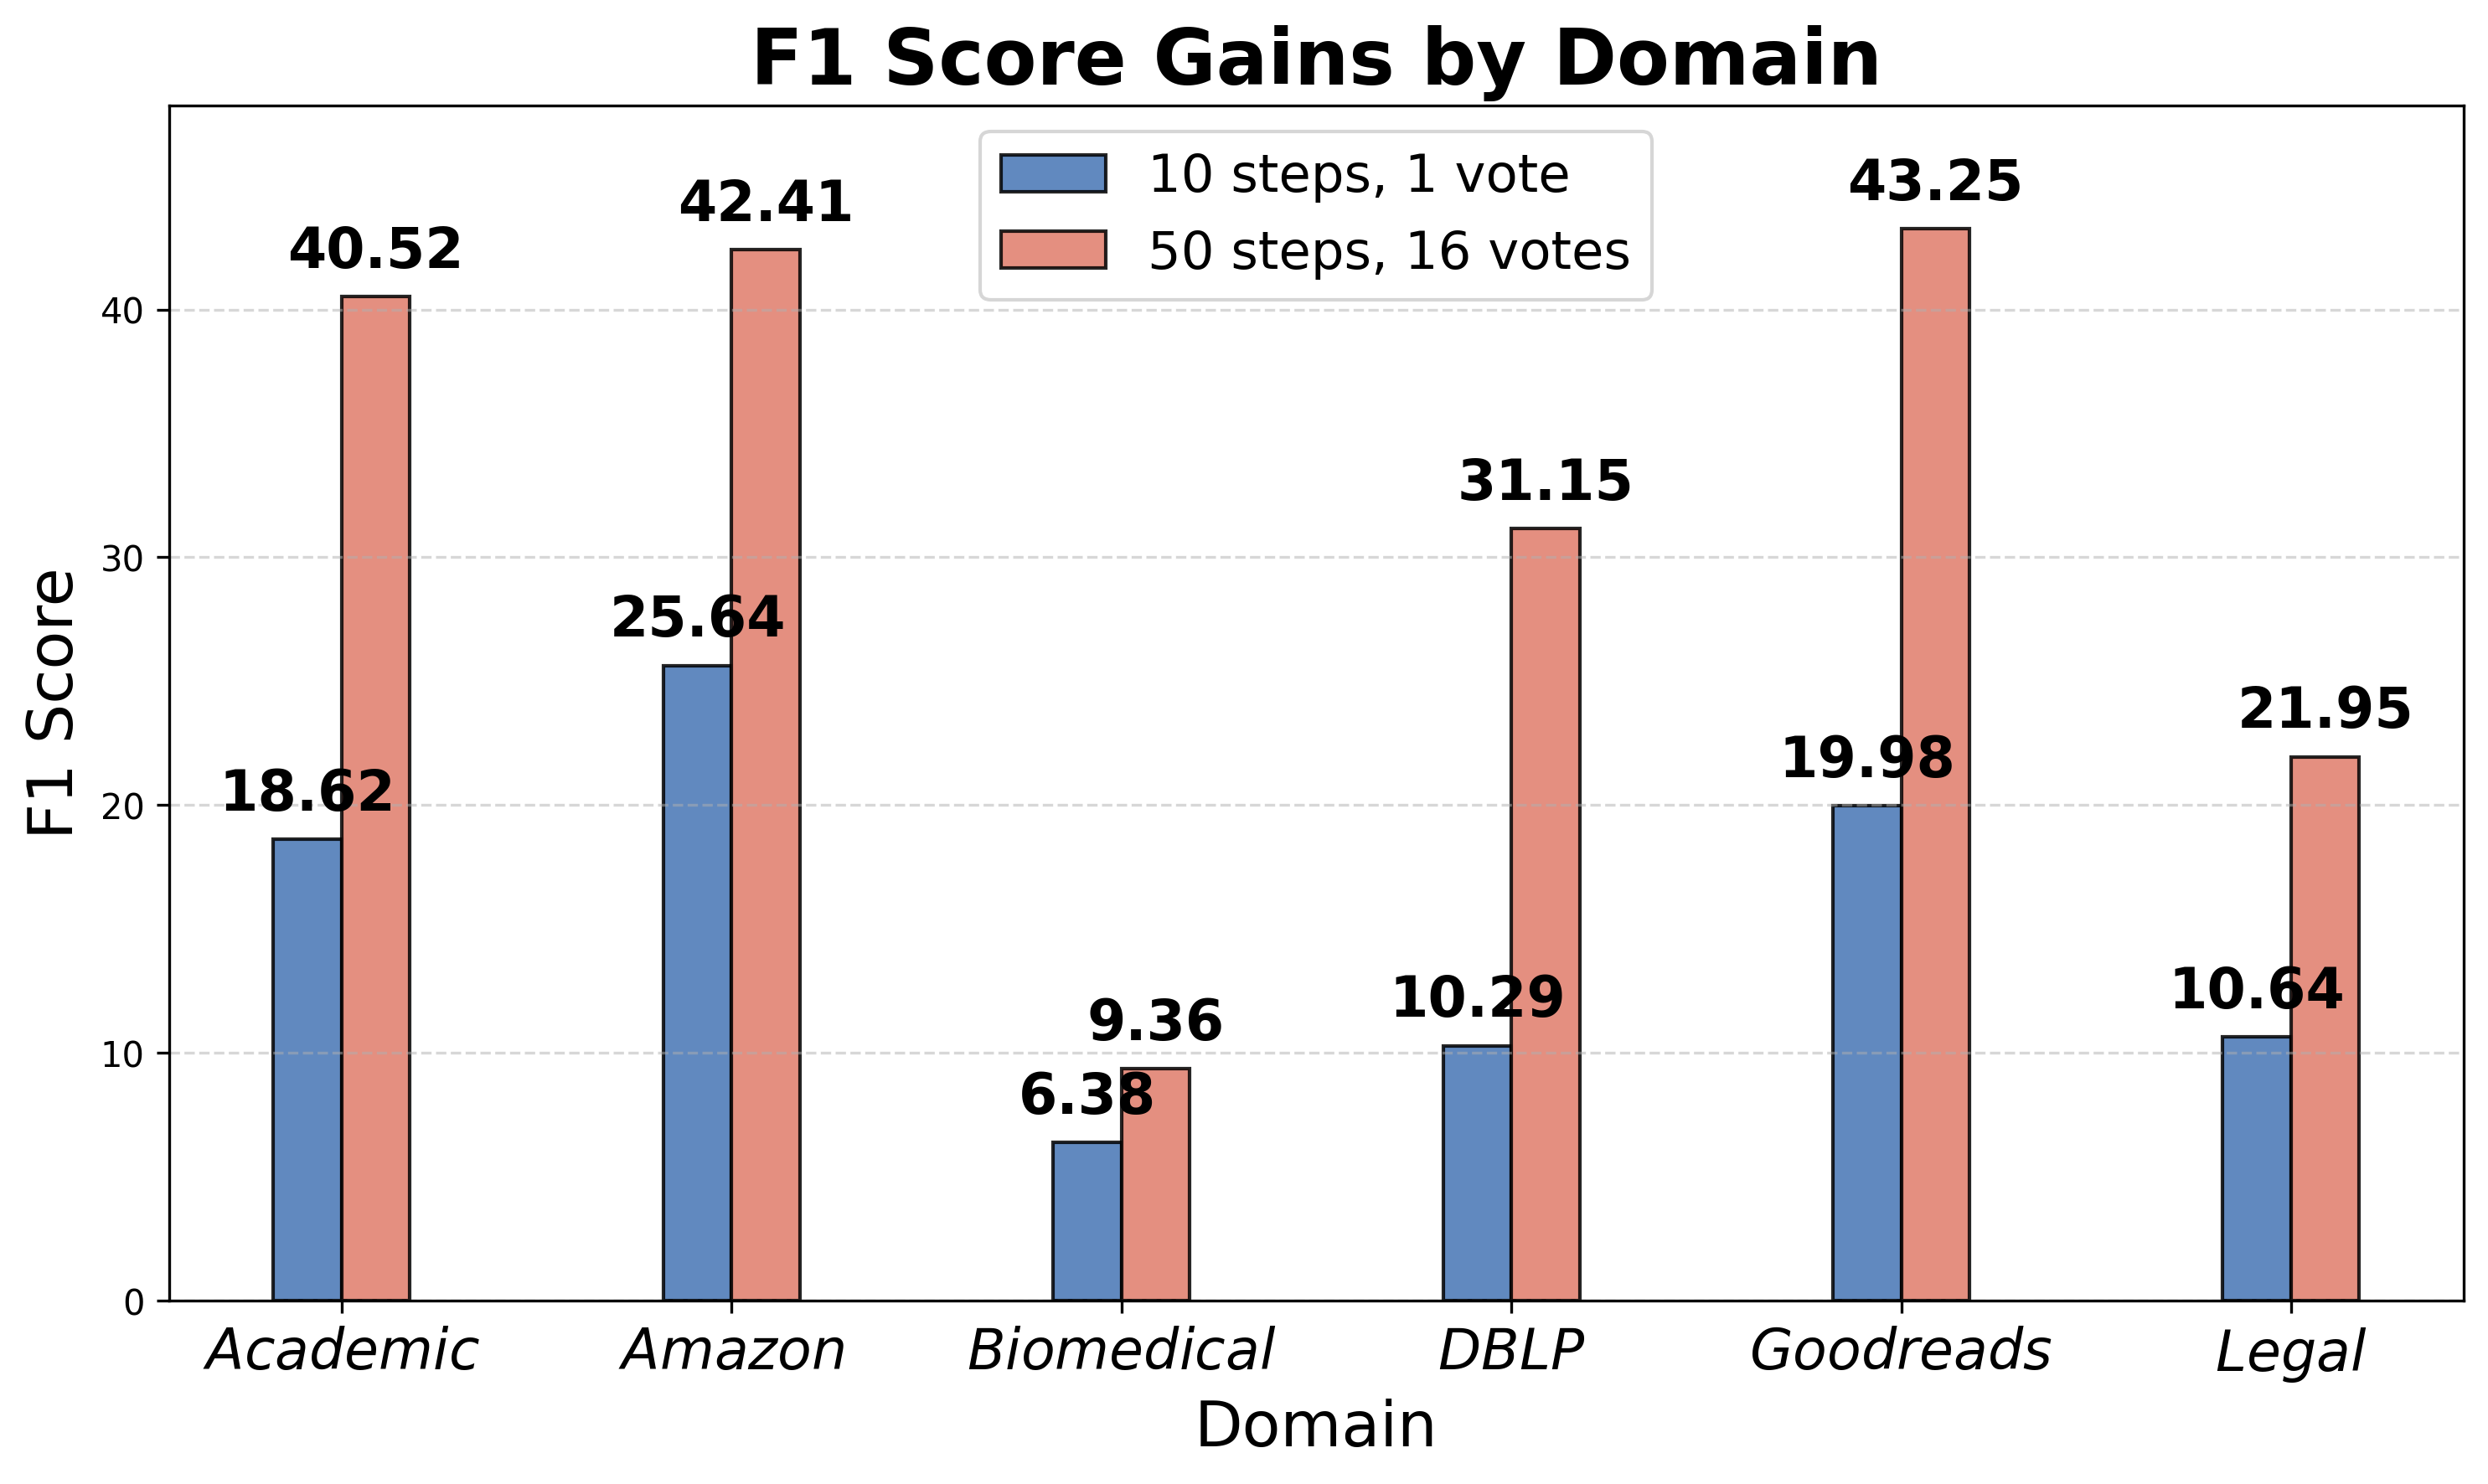
\includegraphics[width=\textwidth]{img/f1_score_medium_hard_avg_domain_bar_chart.png}
        \caption{F1 scores on medium and hard questions}
        \label{fig:multi-hopf1}
    \end{subfigure}
    \begin{subfigure}[t]{0.48\textwidth}
        \centering
        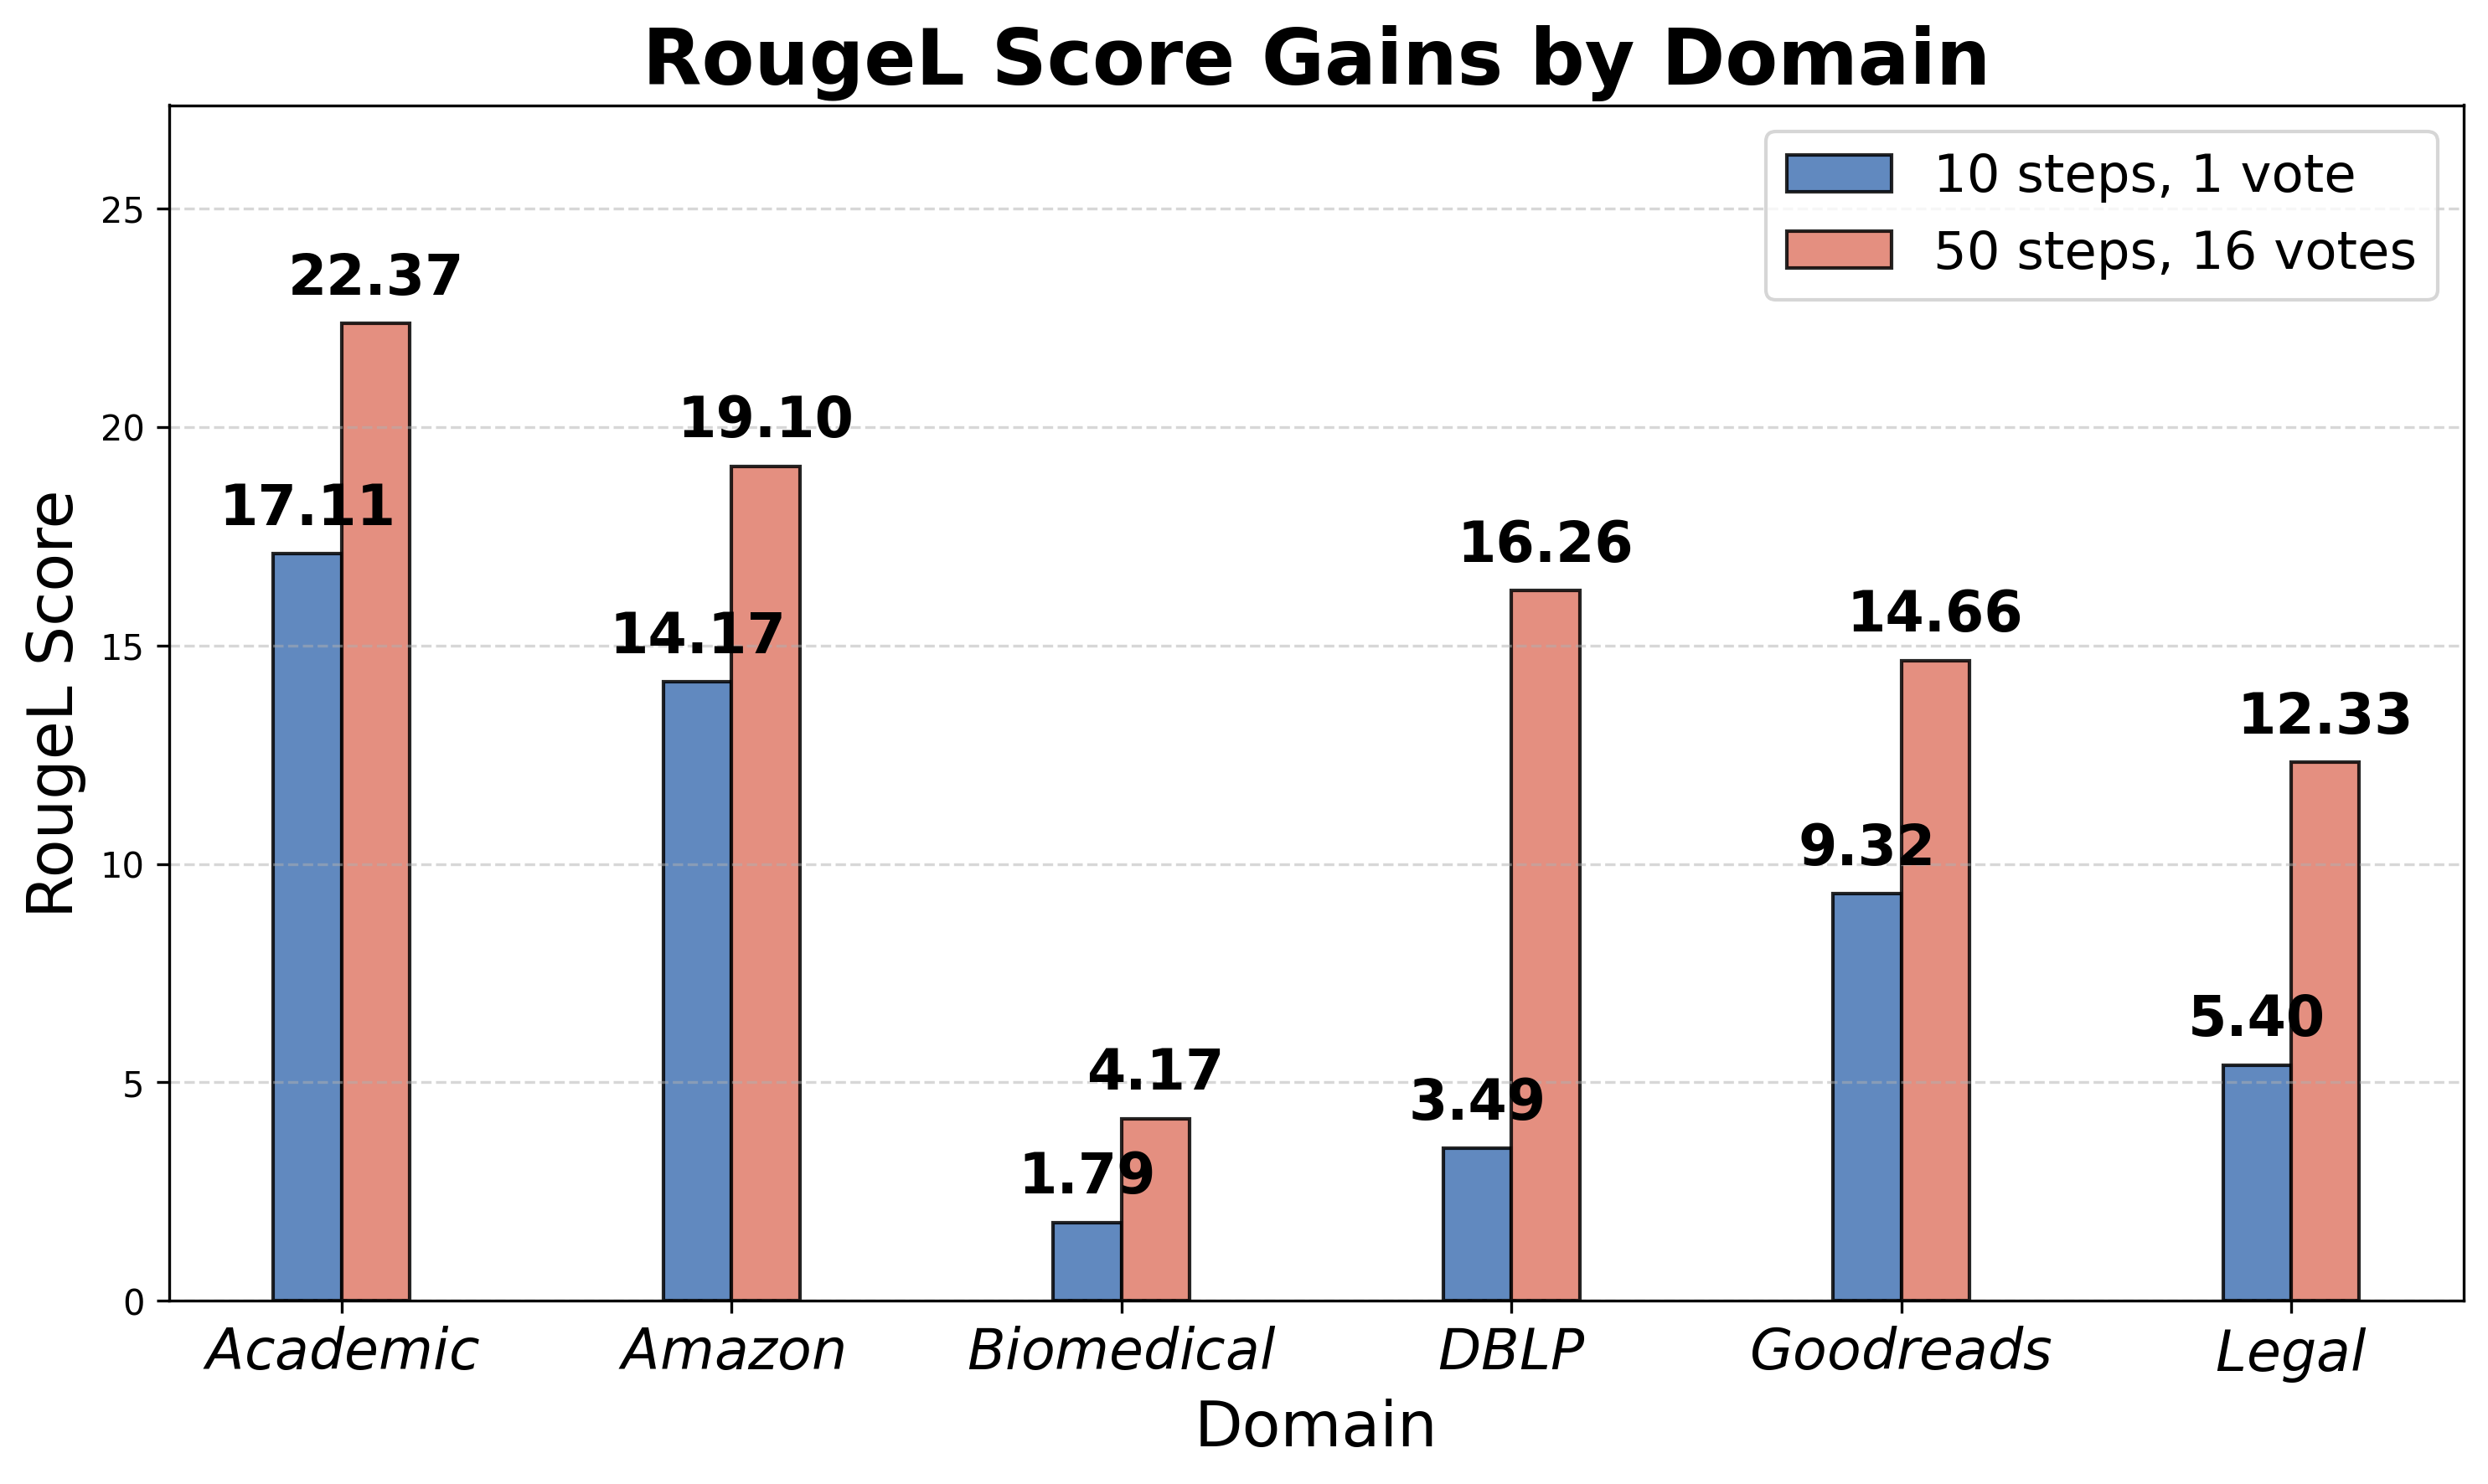
\includegraphics[width=\textwidth]{img/rougel_medium_hard_avg_domain_bar_chart.png}
        \caption{RougeL scores on medium and hard questions}
        \label{fig:multi-hoprougl}
    \end{subfigure}
    \caption{Performance improvements across domains with maximum inference scaling (50 steps, 16 votes) compared to no inference scaling (10 steps, 1 vote). Subfigure (a) reports F1 score gains on medium and hard questions, while (b) shows corresponding improvements in RougeL score. The results demonstrate consistent and substantial gains across all six domains, highlighting the effectiveness of inference scaling for complex question answering }
\end{figure}